\section{Изучение однородности монокристаллов твердого раствора оксида иттрия-европия}

При выборе рефлекса, подходящего для уточнения ПЭЯ \YEu{}, мы столкнулись с проблемой оценки его интенсивности.
Так, например, теоретические значения $F$ рефлексов \hkl(6 8 20) и \hkl(8 6 20), с одинаковым угловым положением $2\theta$, соотносятся как $\approx 7/1$.
Естественно, предпочтительно использовать наиболее интенсивное отражение.
Для решения этой проблемы предварительная съемка кристалла была скорректирована --- расстояние $D$ уменьшено до $60\unit{мм}$, а углы $2\theta_D$ увеличены до $\pm 75\degree$.
В результате были построены сечения обратного пространства (см. рис.~\ref{fig:precession}), захватывающие область углов $2\theta \range{95\degree}{100\degree}$.
Сопоставление интенсивностей рефлексов с результатами вычислений программы James позволило выбрать оптимальные индексы.
По такой схеме было проведено исследование 5 монокристаллов, результаты представлены в табл.~\ref{tab:YEu}. Значения ПЭЯ лежат в интервале от $10.6902\unit{\AA}$ до $10.7045\unit{\AA}$, разница крайних значений составляет $0.0143\unit{\AA}$, что значительно превосходит абсолютную погрешность определения ПЭЯ равную $0.0007\unit{\AA}$.
Таким образом, можно однозначно утверждать, что синтезированный продукт не однороден.

\begin{figure}[ht!]
    \centering
    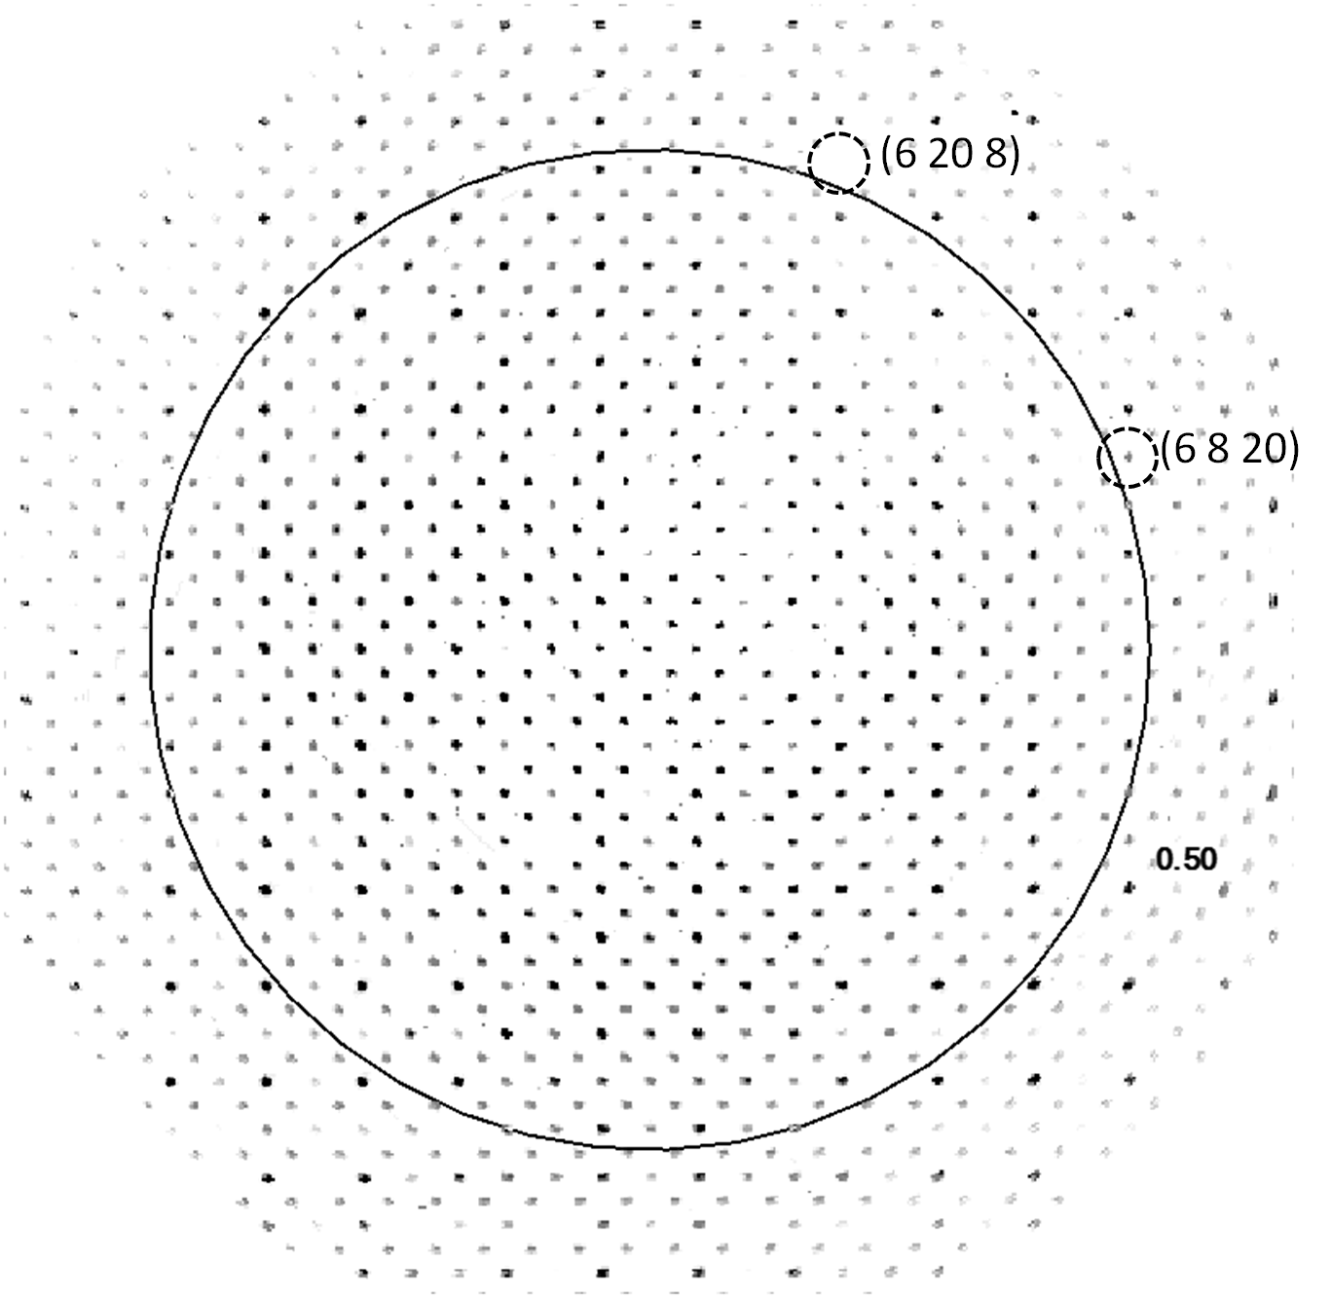
\includegraphics[width=0.8\textwidth]{precession.png}
    \caption{Сечение обратного пространства}%
    \label{fig:precession}
\end{figure}

Для оценки соотношения Y/Eu в изученных монокристаллах можно использовать правило Вегарда.
Для построения соответствующей прямой были использованы литературные данные~\cite{Swanson:1954,Morris:1984,Nikolaev:2023}, а также результаты проведенного нами РСтА 5 кристаллов, отобранных из того же самого продукта синтеза, из которого отобран кристалл $C$ (см. табл.~\ref{tab:YEu} Приложения).
Вместо утерянного кристалла №2 был изучен №6.
Расчет стратегии съемки для накопления полного массива данных производился для каждого кристалла автоматически с учетом его симметрии \hkl(m -3) по предварительно определенной матрице ориентации с использованием пакета программ APEX3.
Далее проводили интегрирование экспериментальных интенсивностей и вводили поправки на поглощение.
Структуры решены с помощью программы ShelxT~\cite{Sheldrick:2015:shelxt} и уточнены с ShelxL~\cite{Sheldrick:2015:shelxl} в графическом интерфейсе Olex2~\cite{Dolomanov:2009}.
Параметры атомных смещений были уточнены в анизотропном приближении.
В результате установлено, что все изученные кристаллы изоструктурны и представляют собой твердые растворы \YEu{}, причем смешанными оказываются обе позиции металла.
Для примера приведем результат исследования кристалла №5: $x = 0.277(10)$, $a = 10.69180(10)\unit{\AA}$, $V = 1222.23(3)\unit{\AA}^3$; пр. гр. $Ia-3$, $Z = 16$, $\rho_\text{выч} = 5.669\unit{г/см}^3$, $\mu_\text{выч} = 38.366\unit{мм}^{-1}$, $F(000) = 1845.0$.
Диапазон сбора данных $2\theta = 7.624-62.84\degree$.
Измерено 4650 отражений $(-11 \leq h \leq 15, -10 \leq k \leq 15, -15 \leq l \leq 10)$.
Независимых рефлексов $N_\text{рефл}/N_\text{рефл} [I > 2\sigma (I)] = 343/340$, $N_\text{параметров} = 19$, $S-\text{фактор}$ по $F^2 = 1.076$; $R_1 [I > 2\sigma (I)]/wR_2 [I > 2\sigma (I)] = 0.0100/0.0224$, $R_1/wR_2 [\text{все данные}] = 0.0101/0.0225$.
Для других кристаллов результаты уточнения аналогичны, диапазон $R_1 [I > 2\sigma (I)]/wR_2 [I > 2\sigma (I)]: 0.0100/0.0224 - 0.0142/0.0313$, $R_1/wR_2 [\text{все данные}]: 0.0101/0.0225 - 0.0152/0.0316$.
Полученные ПЭЯ и $x$ приведены в табл.~\ref{tab:YEu} Приложения.

В результате обработки данных построена прямая $x = -39.96 + 3.77 a_\text{эксп}$~\ref{fig:YEu}.
Значение $x$ для кристаллов, изученных нами по методике Бонда, приведены в табл.~\ref{tab:YEu} Приложения, вместе с данными для кристалла C~\cite{Nikolaev:2023}: все значения $x$ укладываются в достаточно широкий интервал от $\range{0.27}{0.40}$.

\begin{figure}[ht!]
    \centering
    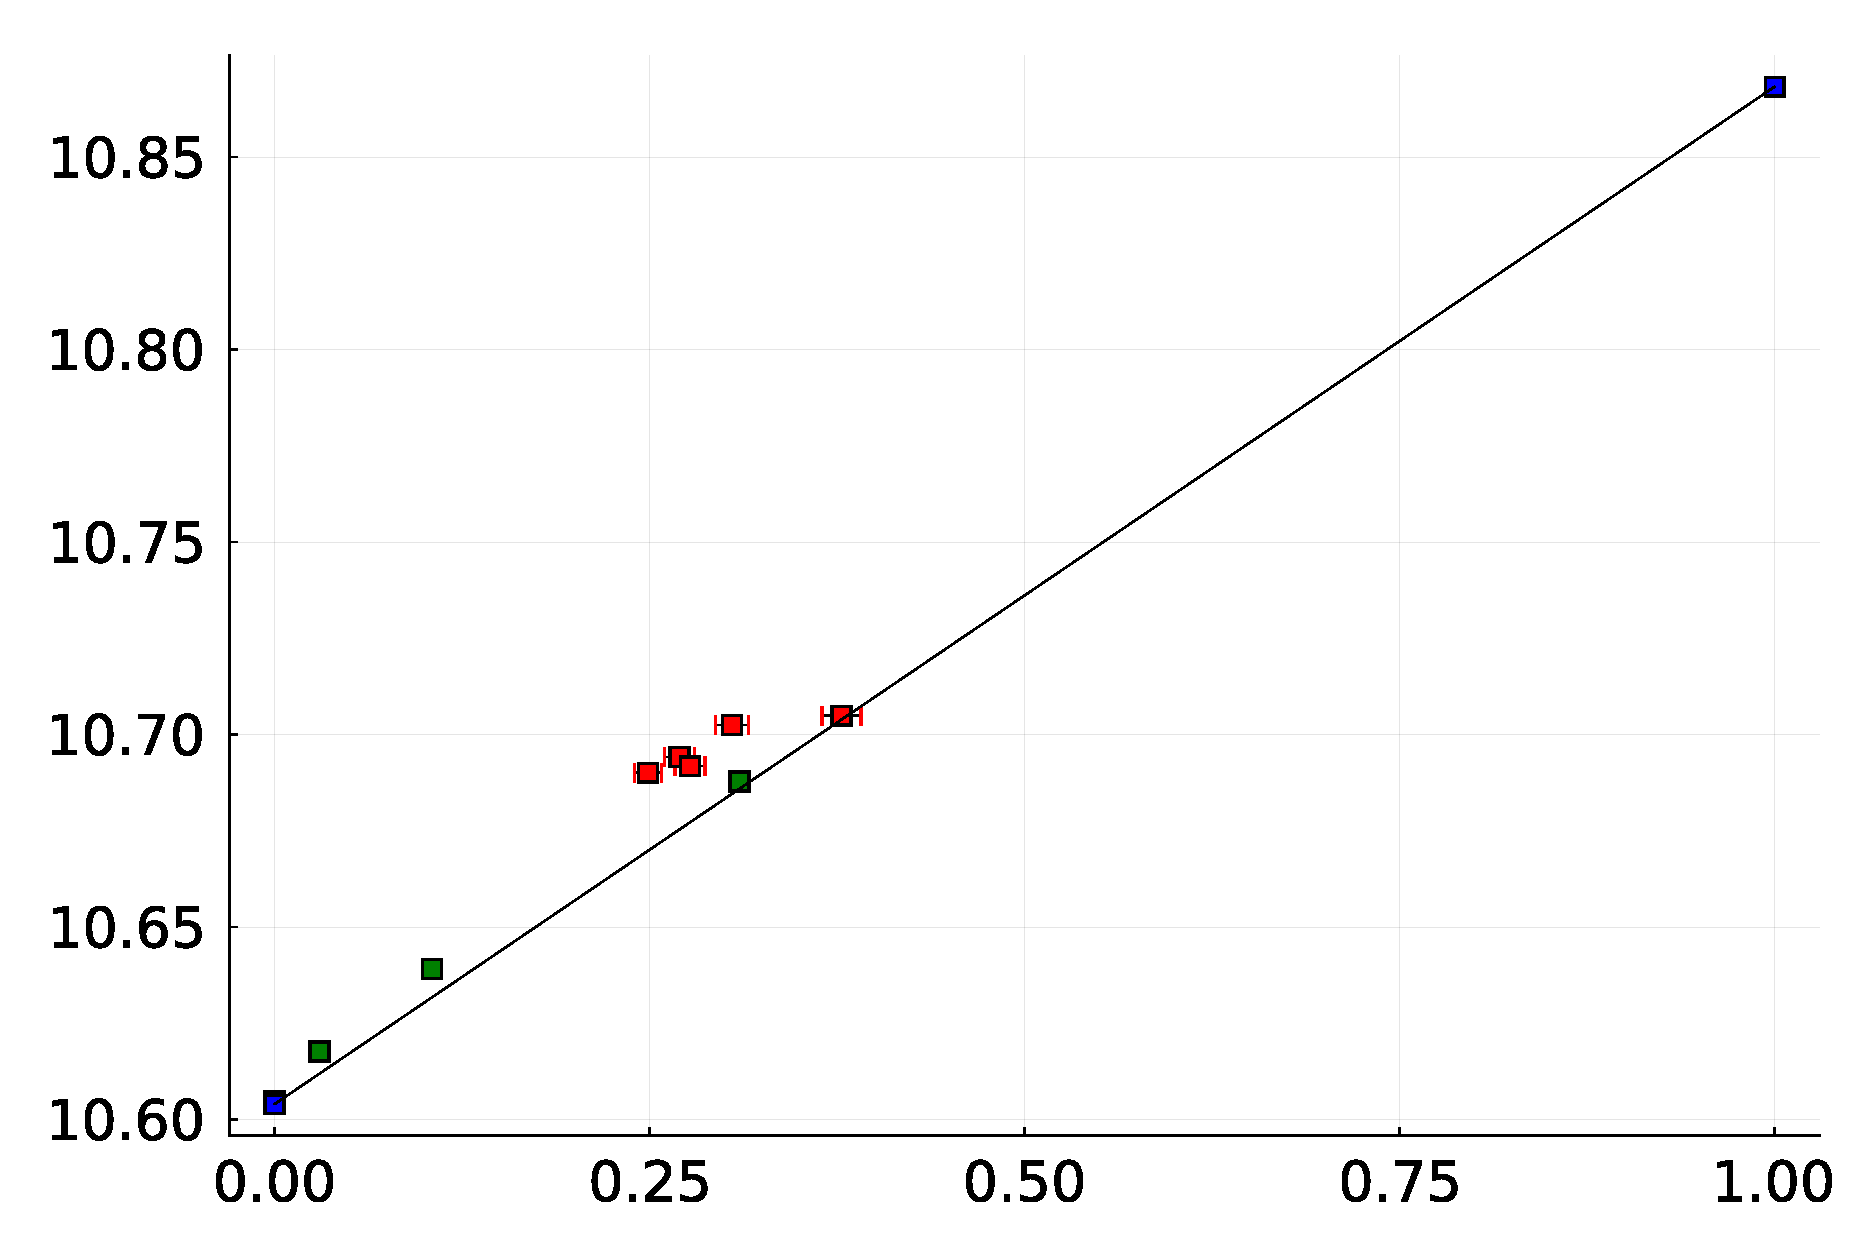
\includegraphics[width=\textwidth]{YEu.pdf}
    \caption{YEu.}%
    \label{fig:YEu}
\end{figure}
